% !TEX root = ./iclr2026_conference.tex
%\section{The Proof Roadmap}

%Για να αποδειξουμε το τελικο bound απαιτουνται πολλα και διαφορετικα στοιχεια που ειναι σπασμενα σε διαφορετικα κομματια που βρισκονται σε διαφορετικα κομματια του appendix. Αρχικα στο appendix C, υπολογιζουμε το convergence rate σε mean squared distance της Perturbed SGD-\RRresh\ μεθοδου. Απο μονο του ως αποτελεσμα εχει το δικο του ενδιαφερον γιατι ειναι μια robustification under noise προηγουμενων αποτελεσματων αλλα στην πραγματικοτητα χτιζει την συναρτηση lyapunov που θα χρειαστουμε για να χειριστουμε την SGD-\RRresh ως ενα διακριτο δυναμικο συστημα μεσω της Markov chain theory in continuous state. Ετσι στο section 3, οπλισμενη με την συναρτηση lyapunov και τις καλες ιδιοτητες του perturbation και την εξυπνη επιλογη να παρατηρουμε per epoch το συστημα, στο appendix D οτι η SGD-\RRresh ειναι μια μαρκοβιανη αλυσιδα που ειναι γεωμετρικα εργοδικη και απολαμβανει ολα τα καλα χαρακτηριστικα: invariant measure/law of large numbers/central limit theorem. Στο Appendix E, θα χρειαστουμε να ελεγξουμε τις 4 ροπες της distance from solution of VIP. Αυτο ειναι ενα τεχνικο δυσκολο task, ειδικα στο section E.2, θα χρειαστουμε να αναπτυξουμε ενα λημμα για τα subset finite sums real vectors και την σταστικη κυρτωση τους (4η ροπη). Ο λογος ειναι για το μεγαλυτερο κομματι της βιβλιογραφιας απαιτει για την \RRrom\ αναλυση και η τεταρτη δυναμη να συμπεριφερεται καλα. (Δες \cite{dieuleveut2020bridging}). Εχοντας κλεισει με αυτο το τελευταιο εργαλειο, στο appendix F δειχνουμε οτι (1) το step-size δεν χρειαζετια να αλλαξει σε ταξη για να κανει η θεωρια accomodate το Εxtrapolation trick φρασοντας της ροπες της ιακωβιανης του induced biased reshuffling gradient estimator. Ειναι η πρωτη φορα που βλεπουμε κατι τετοιο. Τα δυο τελευταια κομματια αυτης της ενοτητας περιλαμβανουν και τις τελικες αποδειξεις του βασικου θεωρηματος του προβληματος. Τελος στο appendix G παρουσιαζουμε μια σειρα απο επιπλεον πειραματα που επιδικνυονυ την πρακτικη υπεροχη της μεθοδου που αποτελεσε και την αφορμη για αυτη την εργασια

\newpage\section{Proof Roadmap}

Our main theorem relies on several technical components, developed across different parts of the appendix.  
In Appendix~\ref{app: convergence_rate}, we establish the mean-squared convergence rate of Perturbed SGD--\RRresh.  
While this result is of independent interest—as it extends prior analyses to a noisy setting—it primarily serves to construct the Lyapunov function that underpins our Markov chain treatment of the algorithm.  
Armed with this Lyapunov function, the properties of the perturbation, and the epoch-level viewpoint, Appendix~\ref{app: efficient_stats} shows that SGD--\RRresh forms a geometrically ergodic Markov chain with all standard consequences: existence of an invariant measure, a law of large numbers, and a central limit theorem.  

Appendix~\ref{app: moments} develops higher-moment control.  
In particular, part~\ref{app: combinatorial} introduces a new combinatorial lemma on fourth moments of finite-sum subsets of vectors—a technically challenging step, motivated by the fact that most extrapolation analyses (e.g., \citet{dieuleveut2020bridging}) require bounded fourth moments of the reshuffling estimator.  
With this tool in hand, Appendix~\ref{app: rich-romberg-proofs} shows that no change in the step-size order is required to accommodate the extrapolation trick: we are able to control the higher moments of the Jacobian of the reshuffled biased gradient estimator.  
To the best of our knowledge, this is the first such result.  
The last parts of Appendix~\ref{app: rich-romberg-proofs} then contain the full proofs of our main theorem.  

Finally, Appendix~\ref{app: additional_experiments} presents additional experiments demonstrating the practical gains of our method, which originally motivated this study.



% --- in preamble ---
\usetikzlibrary{arrows.meta,positioning,fit,shapes,calc}

% \begin{tikzpicture}[node distance=1.8cm,->,>=stealth,thick]
%   \tikzstyle{box} = [rectangle, draw, rounded corners, minimum width=3.3cm, minimum height=1cm, align=center]

%   \node[box] (C) {Appendix C: Convergence rate};
%   \node[box, below=of C] (D) {Appendix D: Markov chain analysis};
%   \node[box, below=of D] (E) {Appendix E: Fourth-moment bounds};
%   \node[box, below=of E] (F) {Appendix F: Extrapolation and bias refinement};
%   \node[box, below=of F] (G) {Appendix G: Additional experiments};

%   % Arrows with slight bends
%   \draw[->] (C) to[bend right=15] (D);
%   \draw[->] (D) to[bend right=15] (E);
%   \draw[->] (E) to[bend right=15] (F);
%   \draw[->] (F) to[bend right=15] (G);

%   % Cross-dependency with bend
%   \draw[->, dashed] (C.east) to[out=0,in=0] (E.east);
%   \draw[->, dashed] (D.west) to[out=180,in=180] (F.west);

% \end{tikzpicture}


\begin{figure}[h]
\centering
\scalebox{0.65}{
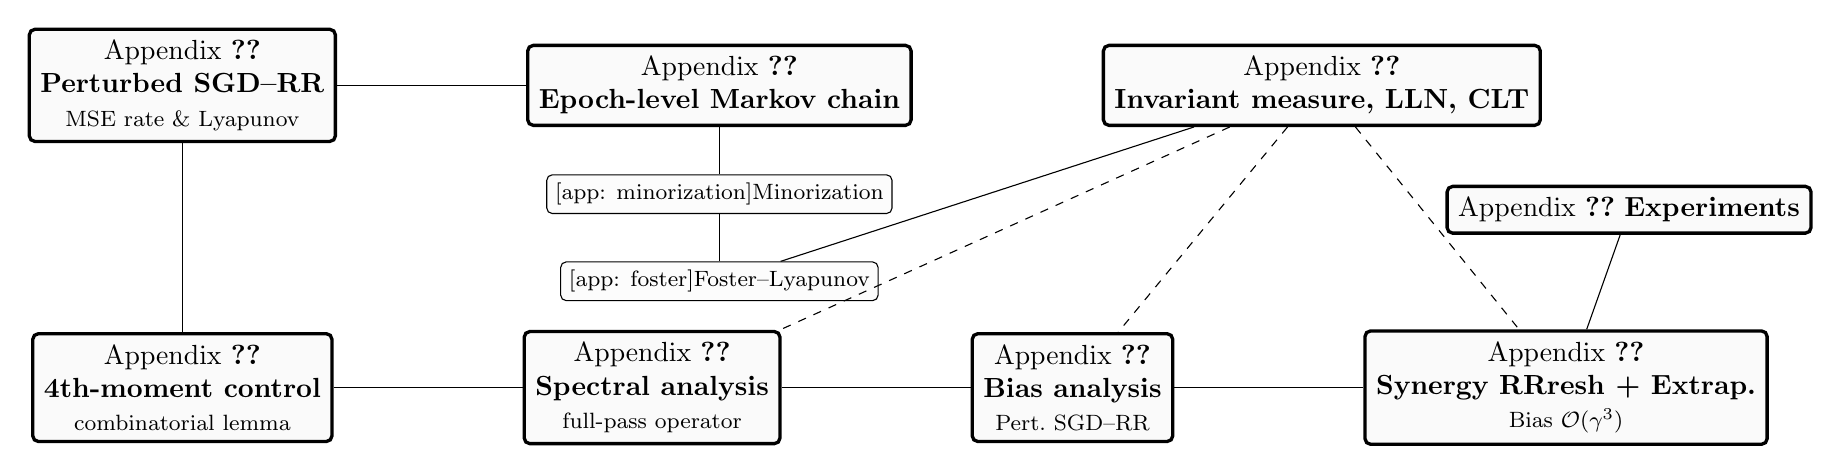
\begin{tikzpicture}[
  node distance=11mm and 16mm,
  >=Latex,
  box/.style={rectangle, rounded corners=2pt, draw=black, very thick, align=center, inner sep=4pt, fill=gray!4},
  small/.style={rectangle, rounded corners=2pt, draw=black, align=center, inner sep=3pt, fill=gray!2, font=\footnotesize},
  every edge/.style={draw=black, -{Latex[length=2.5mm]}}
]


% Appendix C
\node[box] (C1) {Appendix \ref{app: convergence_rate}\\
\textbf{Perturbed SGD--RR}\\
\footnotesize MSE rate \& Lyapunov};

% Appendix D
\node[box, right=24mm of C1] (D1) {Appendix \ref{app: efficient_stats}\\
\textbf{Epoch-level Markov chain}};
\node[small, below=6mm of D1] (D2) {\hyperref[app: minorization]{Minorization}};
\node[small, below=6mm of D2] (D3) {
\hyperref[app: foster]{Foster--Lyapunov}};
\node[box, right=24mm of D1] (D4) {Appendix \ref{app: efficient_stats}\\
\textbf{Invariant measure, LLN, CLT}};

% Appendix E
\node[box, below=24mm of C1, xshift=0mm] (E1) {Appendix \ref{app: combinatorial}\\
\textbf{4th-moment control}\\
\footnotesize combinatorial lemma};

% Appendix F
\node[box, right=24mm of E1] (F1) {Appendix \ref{app: rich-romberg-proofs}\\
\textbf{Spectral analysis}\\
\footnotesize full-pass operator};
\node[box, right=24mm of F1] (F2) {Appendix \ref{app: rich-romberg-proofs}\\
\textbf{Bias analysis}\\
\footnotesize Pert.\ SGD--RR};
\node[box, right=24mm of F2] (F3) {Appendix \ref{app: rich-romberg-proofs}\\
\textbf{Synergy RRresh + Extrap.}\\
\footnotesize Bias $\mathcal{O}(\gamma^3)$};

% Appendix G
\node[box, above=12mm of F3, xshift=8mm] (G1) {Appendix \ref{app: additional_experiments}
\textbf{Experiments}};


% arrows
\draw (C1) -- (D1);
\draw (D1) -- (D2);
\draw (D2) -- (D3);
\draw (D3) -- (D4);

\draw (C1) -- (E1);
\draw (E1) -- (F1);
\draw (F2) -- (F1);

\draw (F2) -- (F3);
\draw (F3) -- (G1);

% dashed auxiliary links
% \draw[dashed] (E1) -- (F3);
 \draw[dashed] (D4) -- (F1);
 \draw[dashed] (D4) -- (F2);
 \draw[dashed] (D4) -- (F3);
\end{tikzpicture}}
\caption{Dependency graph of Appendix results. Solid lines: main logical flow. Dashed lines: auxiliary inputs.}
\label{fig:dep-graph}
\end{figure}

\subsection{Warm-Up:Useful Inequalities}
We start our technical appendix by providing inequalities that will be useful in our proofs
\begin{eqnarray}
		\left\|\sum_{i=1}^n x_i\right\|^2 &\leq& n\sum_{i=1}^n\left\|x_i\right\|^2 \label{ineq1} \\
        \left\|\sum_{i=1}^n x_i\right\|^4 &\leq& n^3\sum_{i=1}^n\left\|x_i\right\|^4 \label{ineqforthefourth}\\
        \left\|a - b\right\|^2 &\geq& \frac{1}{2} \left\|a \right\|^2 - \left\|b\right\|^2 \label{ineqa_b} \\
		\langle a, b \rangle& =& \frac{1}{2} \left[\left\|a \right\|^2 + \left\|b\right\|^2 - \| a-b\|^2\right] \label{ineq inner product} \\
		e^{-x} &\geq& 1 - x, \forall x \geq 0 \label{ineq exponential} \\
            \|a+b\|^2&\leq& \frac{1}{t}\| a \|^2 + \frac{1}{1-t}\|b\|^2, \forall t \in (0, 1) \label{ineq_young_for_t}
\end{eqnarray}
